% Chapter 9

\chapter{Event Selection} % Chapter title

\label{ch:eventsel} 


\begin{table}[htbp]
\begin{center}
 \caption{Overview of all signal, control and validation regions used in the on-shell $Z$ search.
 More details are given in the text.
 %The \met~significance and soft-term fraction $f_{\text{ST}}$ needed in the seed regions for the jet smearing method
 %are defined in Sect.~\ref{sec:zjets}.
 The flavour combination of the dilepton pair is denoted as either ``SF'' for same-flavour or ``DF'' for different flavour.
 All regions require at least two leptons, unless otherwise indicated.
 In the case of CR$\gamma$, VR-WZ, VR-ZZ, and VR-3L the number of leptons, rather than a specific flavour configuration, is indicated.
The main requirements that distinguish the control and validation regions from the signal region are indicated in bold.
Most of the kinematic quantities used to define these regions are discussed in the text. The quantity $m_{\text{T}}(\ell_{3},\met)$
indicates the transverse mass formed by the \met and the lepton which is not assigned to either of the $Z$-decay leptons. }
\resizebox{\textwidth}{!}{
 \begin{tabular}{lcccccccc} %{\textwidth}{@{\extracolsep{\fill}}lcccccccc}
   \noalign{\smallskip}\hline\noalign{\smallskip}
     {\bf On-shell $Z$} &  {\bf \met}   &  {\bf $\htincl$}  &  {\bf $n_{\text{jets}}$}  & {\bf $m_{\ell\ell} $}  &  {\bf SF/DF}  &  {\bf $\Delta\phi(\text{jet}_{12},{\boldsymbol p}\
_{\mathrm{T}}^\mathrm{miss})$ }  &  $m_{\text{T}}(\ell_{3},\met)$ &  $n_{\text{b-jets}}$ \\
     {\bf regions}       &  {\bf [\GeV]} &  {\bf [\GeV]} &                           &    {\bf [\GeV]}        &               &                                             &  [\GeV\
]                        &   \\
   \noalign{\smallskip}\hline\noalign{\smallskip}
   \multicolumn{2}{l}{Signal region} &&&&&& \\
   \noalign{\smallskip}\hline\noalign{\smallskip}
   SRZ  &  $> 225$  &  $> 600$  &  $\geq 2$  & $81 < m_{\ell\ell} < 101$  &  SF  &  $>0.4$ & $-$& $-$\\
   \noalign{\smallskip}\hline\noalign{\smallskip}
   \multicolumn{2}{l}{Control regions} &&&&&&  &  \\
   \noalign{\smallskip}\hline\noalign{\smallskip}
   CRZ              &  $\mathbf{< 60}$   &  $> 600$  &  $\geq 2$   &  $81 < m_{\ell\ell} < 101$       &  SF  & $>0.4$ & $-$  &  $-$ \\
   CR-FS            &  $> 225$  &  $> 600$  &  $\geq 2$   &  $\mathbf{61 < m_{\ell\ell} < 121}$       &  {\bf DF}  & $>0.4$ & $-$  &  $-$ \\
   CRT              &  $> 225$  &  $> 600$  &  $\geq 2$   &  $\mathbf{>40}$, $\mathbf{m_{\ell\ell} \notin [81,101]}$  &  SF  & $>0.4$ & $-$  &  $-$ \\
   CR$\gamma$       &  $-$        &  $> 600$  &  $\geq 2$   &  $-$                                                        &  {\bf $0\ell$, $1\gamma$}  & $-$ & $-$  &  $-$ \\
   \noalign{\smallskip}\hline\noalign{\smallskip}
   \multicolumn{2}{l}{Validation regions} &&&&&& \\
   \noalign{\smallskip}\hline\noalign{\smallskip}
   VRZ  &   $\mathbf{<225}$      &  $> 600$   &  $\geq 2$  &    $81 < m_{\ell\ell} < 101$       &  SF        & $>0.4$  & $-$ & $-$ \\
   VRT  &  {\bf 100--200}     &  $> 600 $  &  $\geq 2$  &    $\mathbf{>40}$, $\mathbf{m_{\ell\ell} \notin [81,101]}$  &  SF        & $>0.4$  & $-$ & $-$ \\
   VRS  &  {\bf 100--200}     &  $> 600 $  &  $\geq 2$  &    $81 < m_{\ell\ell} < 101$       &  SF        & $>0.4$  & $-$ & $-$ \\
   VR-FS & {\bf 100--200}     &  $> 600 $  &  $\geq 2$  &    $\mathbf{61 < m_{\ell\ell} < 121}$  &  {\bf DF}        & $>0.4$  & $-$ & $-$ \\
   VR-WZ  &  {\bf 100--200}   &     $-$      &   $-$        &         $-$                          &  $\mathbf{3\ell}$   &    $-$    & $<100$  &  $0$  \\
   VR-ZZ  &  {\bf $<100$}     &     $-$      &   $-$        &         $-$                          &  $\mathbf{4\ell}$   &    $-$    &  $-$      & $0$   \\
   VR-3L  &  {\bf 60--100}    &  $\mathbf{> 200}$  &  $\geq 2$  &   $81 < m_{\ell\ell} < 101$        &  $\mathbf{3\ell}$   & $>0.4$  & $-$ & $-$ \\
   \noalign{\smallskip}\hline\noalign{\smallskip}
\end{tabular}
} % end of resizebox
\label{tab:regions-z}
\end{center}
\end{table}

\begin{figure}[h]
\centering
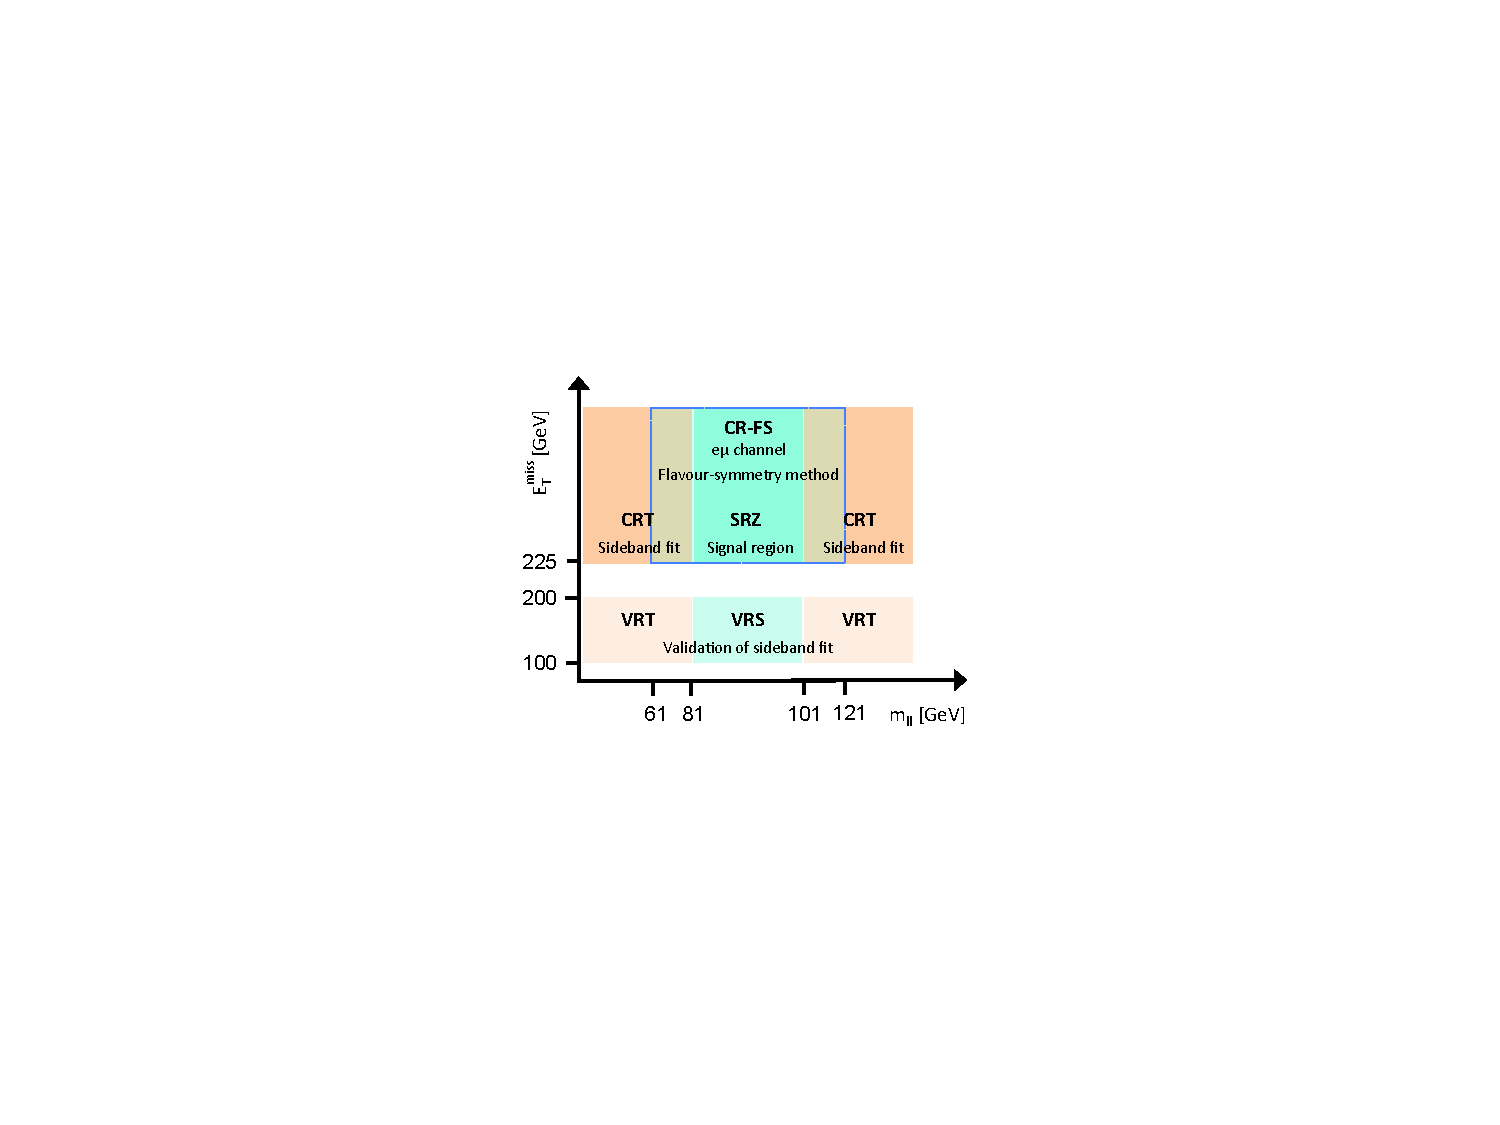
\includegraphics[width=.8\textwidth]{figures/fs/FSdiagram_v2.pdf}\\
\caption{
Schematic diagrams of the control, validation and signal regions for the on-shell $Z$ (top) and edge (bottom) searches.
For the on-shell $Z$ search the various regions are shown in the $\mll-\met$ plane, whereas in the case of the edge search the
signal and validation regions are depicted in the $\HT-\met$ plane.
\label{fig:region_diagrams}
}
\end{figure}

\begin{table}[hbt]
\begin{center}
\begin{tabular}{|lll|}
\hline
Trigger                                       & L1                   & Notes \\ 
\hline\hline
\multicolumn{3}{|l|}{Single electron triggers} \\
\hline
\texttt{HLT\_e60\_lhmedium}                   & \texttt{L1\_EM22VHI} & 2015 and 2016 \\
\texttt{HLT\_e60\_lhmedium\_nod0}             & \texttt{L1\_EM22VHI} & 2016 Only \\
%\texttt{HLT\_e26\_lhtight\_nod0\_ivarloose}   & \texttt{L1\_EM22VHI} & Isolated; for evaluation in 2016 \\
\hline
\multicolumn{3}{|l|}{Di-electron triggers} \\
\hline
\texttt{HLT\_2e12\_lhloose}                   & \texttt{L1\_2EM13VH} & 2015 Only \\
%\texttt{HLT\_2e12\_lhvloose\_nod0\_L12EM10VH} & \texttt{L1\_2EM10VH} & 2016 Only, low-mu \\
%\texttt{HLT\_2e15\_lhvloose\_nod0\_L12EM13VH} & \texttt{L1\_2EM13VH} & 2016 Only, low-mu \\
\texttt{HLT\_2e17\_lhvloose\_nod0}            & \texttt{L1\_EM15VH}  & 2016 Only \\
%\texttt{HLT\_2e17\_lhloose}                  & \texttt{L1\_2EM13VH} &  \\
%\texttt{HLT\_e24\_lhmedium\_e9\_lhmedium}    & \texttt{}            &  \\
\hline\hline
\multicolumn{3}{|l|}{Single muon triggers} \\
\hline
\texttt{HLT\_mu50}                            & \texttt{L1\_MU20}    & 2015 and 2016 \\
%\texttt{HLT\_mu40}                            & \texttt{L1\_MU20}    & Not in MC15a/b \\
%\texttt{HLT\_mu20\_L1MU15}         & \texttt{}   \\
\hline
\multicolumn{3}{|l|}{Di-muon triggers} \\
\hline
\texttt{HLT\_mu18\_mu8noL1}                   & \texttt{L1\_MU15}    & 2015 Only \\
%\texttt{HLT\_2mu10\_nomucomb}                 & \texttt{L1\_MU10}    & 2016 Only, low-mu \\
\texttt{HLT\_2mu14\_nomucomb}                 & \texttt{L1\_MU10}    & 2016 Only \\
%\texttt{HLT\_2mu14}                          & \texttt{L1\_2MU10}       \\
%\texttt{HLT\_mu22\_mu8noL1}                  & \texttt{} \\
\hline
\hline
\multicolumn{3}{|l|}{Electron-muon triggers} \\
\hline
\texttt{HLT\_e17\_lhloose\_mu14}              & \texttt{L1\_EM15VH\_MU10}    & 2015 Only \\
\texttt{HLT\_e7\_lhmedium\_mu24}              & \texttt{L1\_MU20}            & 2015 Only \\
%\texttt{HLT\_e24\_lhmedium\_nod0\_L1EM20VHI\_mu8noL1} & \texttt{L1\_EM20VHI} & 2016 Only, low-mu \\
%\texttt{HLT\_e26\_lhmedium\_nod0\_L1EM22VHI\_mu8noL1} & \texttt{L1\_EM22VHI} & 2016 Only \\
\texttt{HLT\_e17\_lhloose\_nod0\_mu14}        & \texttt{L1\_MU10\_EM15VH}    & 2016 Only \\
\texttt{HLT\_e7\_lhmedium\_nod0\_mu24}        & \texttt{L1\_MU20}            & 2016 Only \\
\hline
\end{tabular}
\caption{
List of the triggers considered for this analysis. The corresponding L1 items are included for reference.  The last column notes if the trigger is available in data.
}
\label{tab:triggerlist}
\end{center}
\end{table}


\begin{table}[hbt]
\begin{center}
\resizebox{1\textwidth}{!}{
\begin{tabular}{|lcc|}
\hline
 %& \hspace*{30mm} \\[-3mm]
Lepton \pt    & Trigger in 2015 & Trigger in 2016    \\
\hline\hline
\multicolumn{3}{|l|}{Di-electron channel} \\
\hline
$\pt(e_1) > 65$~\GeV                               & \texttt{HLT\_e60\_lhmedium} & \texttt{HLT\_e60\_lhmedium\_nod0} \\
$\pt(e_1) \leq 65$~\GeV                            & \texttt{HLT\_2e17\_lhloose} & \texttt{HLT\_2e17\_lhvloose\_nod0} \\
\hline
\multicolumn{3}{|l|}{Di-muon channel} \\
\hline
$\pt(\mu_1) > 52.5$~\GeV                             & \texttt{HLT\_mu50}          & \texttt{HLT\_mu50} \\
$\pt(\mu_1) \leq 52.5$~\GeV                          & \texttt{HLT\_mu24\_mu8noL1} & \texttt{HLT\_2mu14\_nomucomb} \\
\hline
\multicolumn{3}{|l|}{Electron-muon channel} \\
\hline
$\pt(e) > 65$~\GeV                                 & \texttt{HLT\_e60\_lhmedium} & \texttt{HLT\_e60\_lhmedium\_nod0} \\
$\pt(e) \leq 65$~\GeV~and $\pt(\mu) > 52.5$~\GeV     & \texttt{HLT\_mu50}          & \texttt{HLT\_mu50} \\
$\pt(e) \leq 65$~\GeV~and $\pt(\mu) \leq 52.5$~\GeV~and $\pt(e) < \pt(\mu)$  & \texttt{HLT\_e7\_lhmedium\_mu24} & \texttt{HLT\_e7\_lhmedium\_nod0\_mu24} \\
$\pt(e) \leq 65$~\GeV~and $\pt(\mu) \leq 52.5$~\GeV~and $\pt(\mu) < \pt(e)$  & \texttt{HLT\_e17\_lhloose\_mu14} & \texttt{HLT\_e17\_lhloose\_nod0\_mu14} \\
\hline
\end{tabular}
}
\caption{
Lepton trigger requirements used for the analysis in different regions of lepton-\pt\ phase space.
}
\label{tab:trigger_strat}
\end{center}
\end{table}


%----------------------------------------------------------------------------------------

\section{Signal Region}
\label{sec:sr}
\section{Control and Validation Regions}


